\documentclass{article}
\usepackage[utf8]{inputenc}
\usepackage{amsfonts}
\usepackage{listings}
\usepackage{xcolor}
\usepackage{graphicx}
\usepackage{float}
\usepackage{hyperref}

\definecolor{codegreen}{rgb}{0,0.6,0}
\definecolor{codegray}{rgb}{0.5,0.5,0.5}
\definecolor{codepurple}{rgb}{0.58,0,0.82}
\definecolor{backcolour}{rgb}{0.95,0.95,0.92}

\lstdefinestyle{mystyle}{
    backgroundcolor=\color{backcolour},   
    commentstyle=\color{codegreen},
    keywordstyle=\color{magenta},
    numberstyle=\tiny\color{codegray},
    stringstyle=\color{codepurple},
    basicstyle=\ttfamily\footnotesize,
    breakatwhitespace=false,         
    breaklines=true,                 
    captionpos=b,                    
    keepspaces=true,                 
    numbers=left,                    
    numbersep=5pt,                  
    showspaces=false,                
    showstringspaces=false,
    showtabs=false,                  
    tabsize=2
}

\lstset{style=mystyle}

\title{Finite Impartial Combinatorial Game Solver}
\author{Konstantinos Kritharidis}
\date{23/07/2021}

\begin{document}

\maketitle

\section{Introduction}

This document will analyse a code I've written to solve (theoretically) every finite impartial combinatorial game and output an optimal strategy for the winning player. More specifically:
\begin{itemize}
  \item combinatorial game\cite{combinatorial_wiki}: A sequential game with perfect information
  \item impartial\cite{mit}: A game in which the set of allowable moves depends only on the position of the game and not on which of the two players is moving
  \item finite\cite{mit}: There is a finite set of positions available in the game and the game eventually ends
  \item solve: Find if player 1 or player 2 wins
  \item optimal strategy: How the game could evolve assuming the player who had the initial winning position played optimally
\end{itemize}
The code is heavily based on the notes\cite{mit} from MIT on the Theory of Impartial Games which explains how to solve every such game using the Sprague-Grundy Theorem\cite{sg}.

\section{Code Analysis}

\subsection{General Idea}

A game consists of a graph $G = (X, F)$ where\cite{mit}:
\begin{itemize}
\item $X$ is the set of all possible game positions
\item $F$ is a function that gives for each $x \in X$ a subset of possible $x$’s to move to, called followers. If $F(x)$ is empty, the position $x$ is terminal.
\item The start position is $x_0 \in X$. So player 1 moves first from $x_0$.
\item Players alternate moves. At position $x$, the player chooses from $y \in F(x)$.
\item The player confronted with the empty set $F(x)$ loses.
\end{itemize}
We will only look at graphs that are progressively bounded\cite{mit}, meaning that from every start position $x_0$, every path has finite length. In other words, the graph is finite and has no cycles.

The user inputs the initial game state, the possible moves and the terminal states. We construct the graph $G(X, F)$ and calculate the Sprague-Grundy (SG) value of each possible state. If the SG value of the initial state is non-zero, Player 1 wins if they play optimally. Otherwise, Player 2 wins if they play optimally. The code outputs the winning player and proceeds to show a possible winning strategy by starting at the initial state and climbing down the graph.

Assuming player 1 wins if they play optimally, we travel to a state which has an SG value of zero. Then, regardless of which move Player 2 makes, they are destined to lose, if Player 1 plays optimally, so they make a random move. The process repeats until a terminal state is reached. There, Player 2 will have no possible move and will, thus, lose the game. 

\section{Challenges}

\subsection{Range of games}

There are two challenges for the further development of this game solver. The first is to make it solve more types of games. Even though it should be able to solve every finite impartial combinatorial game, due to the way the user inputs the possible moves, the code can't solve games in which there are more complex restrictions in the moves that a player can make (eg. only subtract numbers that divide the current number in one of the heaps).
\begin{figure}[H]
\centering
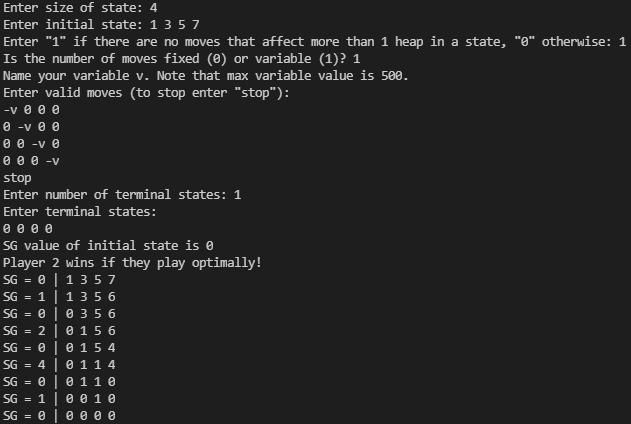
\includegraphics[scale=0.75]{nim}
\caption{Example of the nim game with 4 heaps}
\label{fig:nim}
\end{figure}

To solve that first challenge, we should be able to add more complex restrictions on the variable v shown above. For example the first row during the moves input would be "-v 0 0 0 v $\mid$ a{\_}1", where a{\_}1 would denote the current number in the 1st heap and $\mid$ is the divides symbol. The code should be able to understand that grammar, as well as all other possible restrictions the user should wish to add.

\subsection{Space and Time Complexity}

\subsubsection{Problem}

The second challenge is reducing the space and time complexity of the algorithm. Currently, due to the fact that the algorithm creates all possible game states $x$ and stores them in a graph $G(X, F)$, both the space and time complexity of the algorithm is exponential with regard to the size of the input.

That can be easily seen through the nim example as shown in Figure \ref{fig:nim}. Since the graph will contain all possible game states, the set $X$ of its nodes will be the set of all quadruplets whose ordered elements are less than or equal to the respective ordered elements in the initial state. Therefore, if we let $P = \prod_{i=1}^4 a_i$, the complexity of the algorithm will be $O(P)$. If we let $M$ be the size of the input then $M = \sum_{i=1}^4 \log a_i = \log P \Leftrightarrow P = 2^M$, so the complexity is $O(2^M)$.

The fact that the complexity is that high, means that we can't solve games in which the initial state is too large (ie. the set of possible game states is too large). To solve that problem, both the space and time complexity of the algorithm need to be reduced.

\subsubsection{Improvement for a certain type of games}

Currently, there is an optimization for games that can be represented as the sum of disjoint sub-games. Such a game contains moves that only affect one heap at a time. There, by making use of the theory for \hyperref[subsec:gameSum]{sums of games}, we can solve the distinct sub-games and then combine the answers (function solve()), instead of solving the total game on its own. In this way, if we let $S = \sum_{i=1}^4 a_i$ we can solve the game in $O(S)$ and output the optimal strategy (function strategy()) in $O($depth$ \cdot $no.{\_}of{\_}moves), where depth is the number of turns played in the game until it ends and no.{\_}of{\_}moves is the number of available moves to go from one state of the game to another.

Suppose we have a sum-game of $N$ disjoint sub-games of size 1 which all have the same number $a$ in their heap and the only moves are to subtract 1 or 2 from one heap (so there are $\Theta(2N) = O(N)$ moves available). Then the size of the input is $M = \sum_{i=1}^N \log a = N \log a \Leftrightarrow a = 2^{\frac{M}{N}}$. Then, $S = N \cdot a$, so the complexity of solve() becomes $O(N \cdot a) = O(N \cdot 2^{\frac{M}{N}})$. The SG values in each heap are periodic with a period of 3. Each game can finish in $\Theta(\frac{a}{3}) = O(a)$ moves, while the optimal strategy could be achieved by only playing at 1 heap until it ends, since the player will always be able to make the total nim-sum 0 regardless of the heap, so the total depth $= \Theta(\frac{2}{3} \cdot N \cdot a) = O(N \cdot a)$ and the complexity of strategy() is $O(N \cdot a \cdot N) = O(N^2 \cdot a) = O(N^2 \cdot 2^{\frac{M}{N}})$.

In a normal nim game, if all heaps have the same number $a$, the complexity of solve() stays the same, $O(S) = O(N \cdot a) = O(N \cdot 2^{\frac{M}{N}})$. The complexity of strategy(), on the other hand, becomes more complex, since the depth isn't that trivial, although it is certainly much smaller than $O(N \cdot a) = O(S)$ which was the depth in the previous example. The no.{\_}of{\_}moves, however, increases, since in each state it is $O(S)$. Thus, the overall complexity of strategy() will be much smaller than $O(S^2) = O(N^2 \cdot a^2) = O(N^2 \cdot 2^{\frac{2M}{N}})$. A better upper-bound for the complexity of strategy() in that case remains to be found.

\section{Notes\cite{mit}}

\subsection{Sprague-Grundy Function}

To analyze the game we will need to use the function $mex$, or minimum excluded value, defined as
$$mex(S) = min{\{}n \in \mathbb{N} : n \notin S{\}}$$
The Sprague-Grundy function of a graph G = (X, F) is a function $g$ defined on $X$ that takes only non-negative integer values and is computed as follows:
$$g(x) = mex{\{}g(y) : y \in F(x){\}}$$
In words, the Sprague-Grundy (SG) is the smallest non-negative value not found among the SG values of the followers of $x$.

Since this function is defined recursively, we’ll need some base cases. We set all terminal nodes $x$ to have $g(x) = 0$. Then any nodes that have only terminal nodes as followers have $g(x) = 1$. In this way we can work our way through the graph until all nodes are assigned an SG value.

\subsection{Sum of Games}
\label{subsec:gameSum}

We can add any $n$ games $G_i$ together as follows:\\
To sum the games $G_1 = (X_1, F_1), G_2 = (X_2, F_2), \dots, G_n = (X_n, F_n)$,\\
$G(X, F) = G_1 + G_2 + \dots + G_n$ where:
\begin{itemize}
\item $X = X_1 \times X_2 \times X_3 \times \dots \times X_n$, or the set of all $n$-tuples such that $x_i \in X_i \forall i$
\item The maximum number of moves is the sum of the maximum number
of moves of each component game.
\end{itemize}

According to the Sprague-Grundy Theorem, the SG function for a sum of games on a graph is just the Nim sum of the SG functions of its components.\\
If $g_i$ is the Sprague-Grundy function of $G_i, i = 1, \dots, n$, then $G = G_1 + \dots + G_n$ has Sprague-Grundy function $g(x_1, \dots, x_n) = g_1(x_1) \oplus \dots \oplus g_n(x_n)$.

The winning strategy on a game that can be represented in such a graph would be to move to a vertex with $g(x) = 0$.

\begin{thebibliography}{9}

\bibitem{combinatorial_wiki} 
Combinatorial game theory, Wikipedia
\\\texttt{https://en.wikipedia.org/wiki/Combinatorial{\_}game{\_}theory}

\bibitem{mit} 
Theory of Impartial Games, MIT
\\\texttt{http://web.mit.edu/sp.268/www/nim.pdf}

\bibitem{sg} 
Sprague–Grundy theorem, Wikipedia
\\\texttt{https://en.wikipedia.org/wiki/Sprague-Grundy{\_}theorem}

\end{thebibliography}

\end{document}
